%% LaTeX2e class for student theses
%% sections/content.tex
%% 
%% Karlsruhe Institute of Technology
%% Institute for Program Structures and Data Organization
%% Chair for Software Design and Quality (SDQ)
%%
%% Dr.-Ing. Erik Burger
%% burger@kit.edu
%%
%% Version 1.3.3, 2018-04-17

\chapter{Introduction}
\label{ch:Introduction}
\section{Motivation}
\label{sec:Introduction:Motivation}
Correlation analysis aims at discovering and summarizing the relationship between the attributes of a data set. Knowing the relationship between a set of variables, one can infer useful knowledge about external, a priori unknown outcomes.\\
For example, we can measure the stock relationship via correlation coefficients in stock markets that may undergo large fluctuations of stock prices. The representing of the correlation coefficients among the five funds’ returns from 1980 to 1998 by Katrina Simons is shown in \autoref{fig:correlations}. Correlation coefficients describe the extent to which asset returns “move together.” Correlation coefficients range in value between negative one (completely negatively correlated) and positive one (completely positively correlated), while a correlation of zero means that there is no correlation between two attributes. Performing good correlation analysis could be of great help to a financial analysis.\\
\begin{figure}[h]
	\centering
	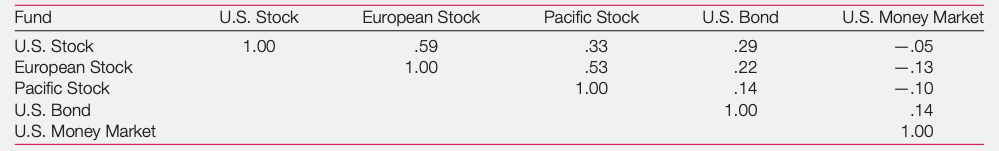
\includegraphics[width=\textwidth]{pictures/motivation1}
	\caption{Correlations Among the Five Funds’ Returns, Monthly Returns, from 1980 to 1998\cite{simons1999should}}
	\label{fig:correlations}
\end{figure}\\
We can see that the stock markets are positive correlated between each other, which indicates a similar behavior during this period. If we are fully aware of our current stock market, we are likely to predict the behavior of other stock markets due to the positive correlation. As a result, if we know that one stock market is performing well, we can maximize our wealth by investing other stock markets, which are positive correlated to our current stock market. If we want to minimize the risk of investing, it's better to invest in no correlated stock markets.
\begin{figure}[h]
	\centering
	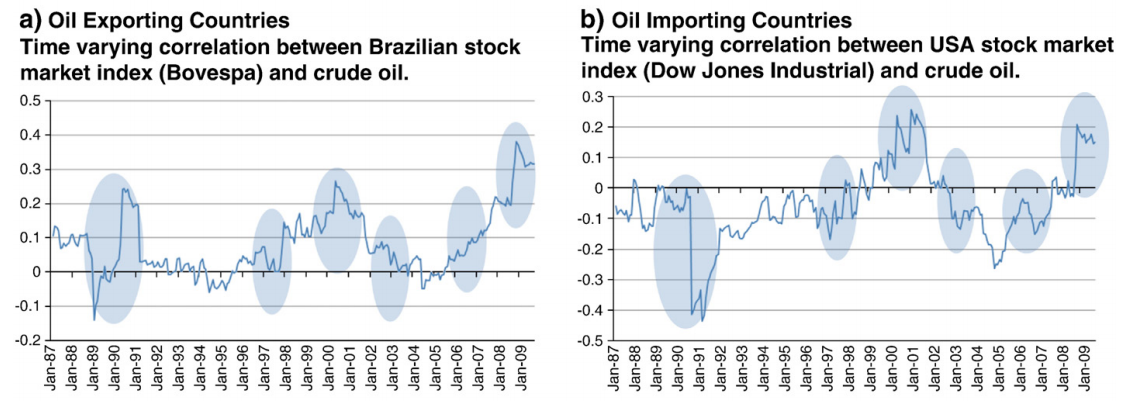
\includegraphics[width=\textwidth]{pictures/motivation21}
	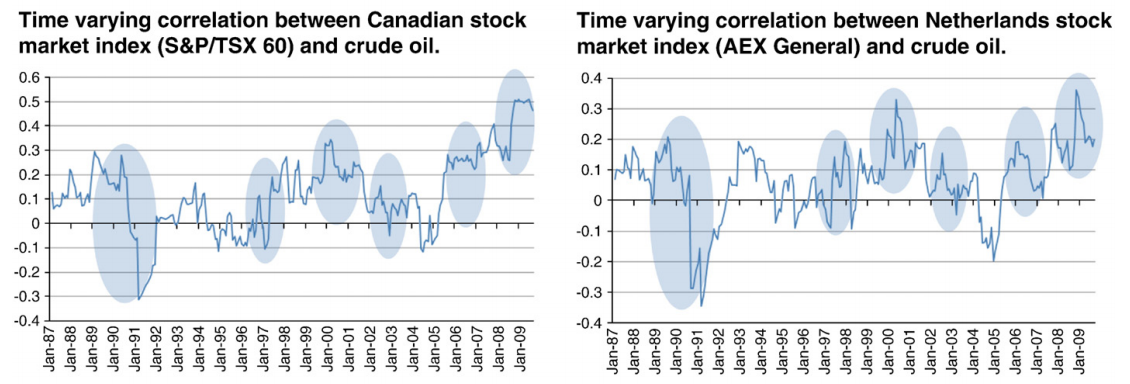
\includegraphics[width=\textwidth]{pictures/motivation22}
	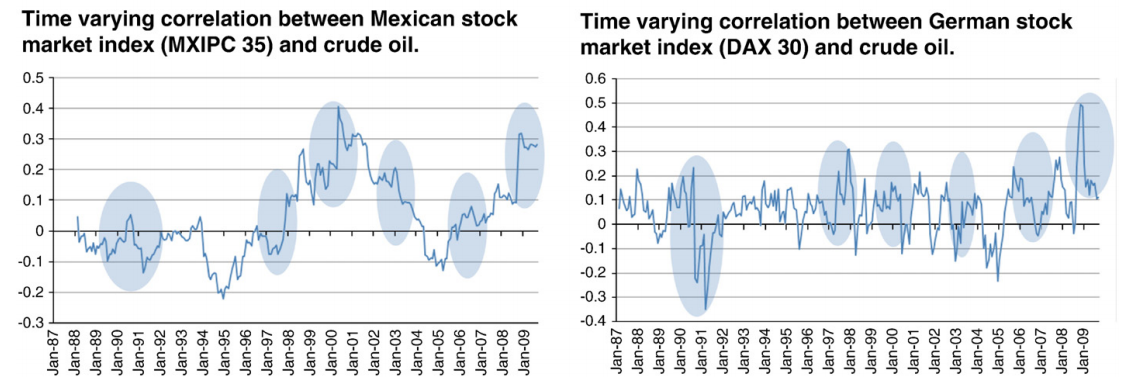
\includegraphics[width=\textwidth]{pictures/motivation23}
	\caption{Dynamic correlation between stock market index and the crude oil price\cite{FILIS2011152}}
	\label{fig:brutal}
\end{figure}\\
Analyzing the correlation between different attributes helps us to understand their relationship. In general, the correlations between attributes remain same or change gradually. If the correlation structure changes brutally, which often indicates a sudden peak or valley, we can infer that one of the attributes may have an enormous change or the relationship between them may differ thoroughly.
George Filis et al. analyzed in \cite{FILIS2011152} the dynamic correlation between stock market index and the crude oil price, which is shown in \autoref{fig:brutal}. During the period 1987 - 2009, 6 important events occurred: 
\begin{itemize}
	\item Iraq invasion in Kuwait/first war in Iraq
	\item Asian economic crisis
	\item Housing market boom
	\item Second war in Iraq
	\item Chinese economic growth
	\item Global financial crisis
\end{itemize}
These events signed the brutal changes in the correlation between markets and oil price, which are printed in blue circles in the \autoref{fig:brutal}.\\

\section{Challenges}
\label{sec:Introduction:Challenges}
The challenges of analyzing high-dimensional data streams is twofold: the evolving nature of streams and the high-dimensionality.\\

\subsection{The evolving nature of streams}
\label{sec:Introduction:Challenges:Streams}
In contrast to static data, the data is often available as a stream, i.e., it is an infinite, ever evolving sequence of observations. As the concepts learned at a certain time cannot be expected to hold in the future, correlation analysis should be a continuous process. We can see from \autoref{fig:brutal} that the correlation between market and oil price is always changing throughout the time. The correlation values even have brutal changes, when meet up with important events. Therefore, it's quite hard for the data scientists to predict the correlation value at next timestamp.\\

\subsection{The high-dimensionality}
\label{sec:Introduction:Challenges:High-dimensionality}
Also, the data is often high-dimensional, i.e., it contains hundreds or thousands of dimensions. In the case of streams with many dimensions, it is difficult to extract actionable insights from the correlation matrix, as the number of pairs of attributes increases quadratically and the coefficients evolve over time in unforeseen ways. For the pairwise correlation analysis of any data steam with $n$ components, one need to compute the correlation between $ \dfrac{n*(n-1)}{2} $ pairs, i.e., with $ n=5 $, one needs to compute 10 pairs, with $ n=10 $, one needs to compute 45 pairs. Therefore, it becomes difficult to visually keep track of correlation and impossible to understand the result of the correlation analysis as the number of attributes increases. The \autoref{fig:visualization} shows the visualization of different numbers of attributes. As an instance, with the developing number of attributes, it becomes even harder for users to compare the correlation value between two pairs using Heatmap as the standard tool to visualize the data.\\
\begin{figure}[h]
	\centering
\begin{subfigure}[b]{0.3\textwidth}
	\centering
	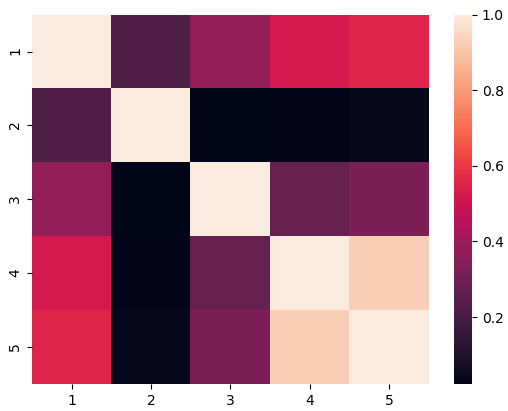
\includegraphics[width=\textwidth]{pictures/bioliq5}
	\caption{Correlation matrix of 5 attributes}
	\label{fig:matrix5}
\end{subfigure}
\hfill
\begin{subfigure}[b]{0.3\textwidth}
	\centering
	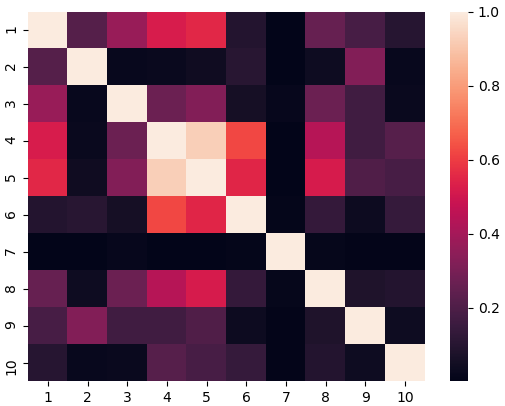
\includegraphics[width=\textwidth]{pictures/bioliq10}
	\caption{Correlation matrix of 10 attributes}
	\label{fig:matrix10}
\end{subfigure}
\hfill
\begin{subfigure}[b]{0.3\textwidth}
	\centering
	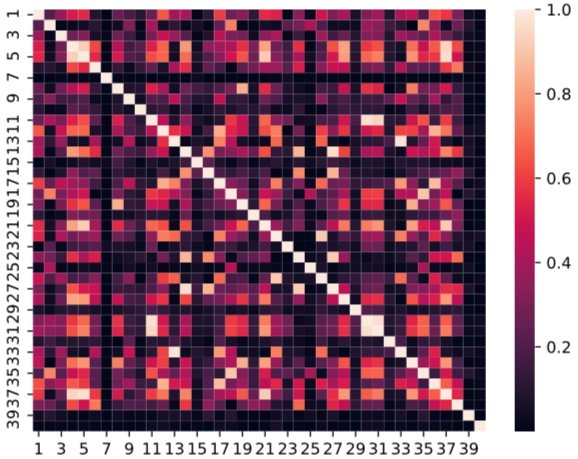
\includegraphics[width=\textwidth]{pictures/bioliq40}
	\caption{Correlation matrix of 40 attributes}
	\label{fig:matrix40}
\end{subfigure}
	\caption{Visualizations of different numbers of attributes}
	\label{fig:visualization}
\end{figure}
\section{Goal of the thesis}
\label{sec:Introduction:GoalOfTheThesis}
The goal of this thesis is to propose and evaluate new tools for the interactive visualization of correlation in high-dimensional streams. We are going to compare different visualization methods. Our interactive interface aims at providing a visualization of correlations in streams, which may change arbitrarily over time, for people. Users are able to choose a certain period of time to perform the correlation analysis and visualization. In our thesis, we only focus on pairwise relationships and the correlations between more than two variables may remain to be discovered in the future work. We are going to answer the following three questions in the thesis:
\begin{itemize}
	\item What visualization method is the most appropriate to visualize correlation for various specific user information needs?
	\item What visualization method is the most suitable to visualize characteristics of a data set?
	\item What are the desirable features of a correlation monitoring interface?
\end{itemize}
To answer these questions, we first search for three interactive visualization methods and then develop an interface to visualize correlations using these methods. This interface can be available in a browser and should be user friendly, which means that users provide their own data sets and the system’s back-end calculates the correlations and then provides the visualization of the results. Users are also able to interact in several ways with this interface, such as setting parameters to tune the visualization. At last, we evaluate the benefits of our interface systematically via controlled user studies and discuss the advantages and disadvantages of each visualization method when meet up with different scenarios. Based on the results, we discover the appropriate visualization methods of correlations in high-dimensional streams and the desirable features of the interactive interface.\\
\section{Thesis outline}
\label{sec:Introduction:ThesisOutline}
This thesis is divided into three parts: the literature review of visualization methods, the design and implementation of interface, and the evaluation of this interface.\\
In \autoref{ch:Visualization}, the first part of the thesis, we introduce three state-of-art methods for correlation visualization: Heatmap, Bar Graph and Force-Directed-Graph.\\
\autoref{ch:RelatedWork} is about the related work. In \autoref{ch:RelatedWork}, we give an overview\cite{Matrics} of parallel coordinates and scatterplot matrices as examples of multidimensional visualization techniques. Also, we introduce an interactive Framework for Exploring and Understanding Multivariate Correlations "FEXUM"\cite{FEXUM} created by Louis Kirsch et al., which uses Force-Directed-Graph as the visualization method for the data set.\\
\autoref{ch:Interface} is the main part of this thesis. \autoref{sec:Interface:Design} is the design of the interface and \autoref{sec:Interface:Implementation} describes the implementation of this interface.\\
We evaluate the developed interface in \autoref{ch:Evaluation}. It contains not only the experimental settings of controlled user studies for evaluation in \autoref{sec:Evaluation:ExperimentalSettings}, but also the results of controlled user studies and feedbacks in \autoref{sec:Evaluation:Result}.\\
The summary of the whole thesis comes in the end.\\